%
%                       This is a basic LaTeX Template
%                       for the Informatics Research Review

\documentclass[a4paper,11pt]{article}
% Add local fullpage and head macros
\usepackage{head,fullpage}     
% Add graphicx package with pdf flag (must use pdflatex)
\usepackage[pdftex]{graphicx}  
% Better support for URLs
\usepackage{url}
% Date formating
\usepackage{datetime}

\newdateformat{monthyeardate}{%
  \monthname[\THEMONTH] \THEYEAR}

\parindent=0pt          %  Switch off indent of paragraphs 
\parskip=5pt            %  Put 5pt between each paragraph  
\Urlmuskip=0mu plus 1mu %  Better line breaks for URLs


%                       This section generates a title page
%                       Edit only the following three lines
%                       providing your exam number, 
%                       the general field of study you are considering
%                       for your review, and name of IRR tutor

\newcommand{\examnumber}{B240710}
\newcommand{\field}{Network Science Analysis : An Elixir to Prevent Global Financial Crisis?}
\newcommand{\supervisor}{Xinran Ruan}

\begin{document}
\begin{minipage}[b]{110mm}
        {\Huge\bf School of Informatics
        \vspace*{17mm}}
\end{minipage}
\hfill
\begin{minipage}[t]{40mm}               
        \makebox[40mm]{
        \includegraphics[width=40mm]{crest.png}}
\end{minipage}
\par\noindent
    % Centre Title, and name
\vspace*{2cm}
\begin{center}
        \Large\bf Informatics Research Review \\
        \Large\bf \field
\end{center}
\vspace*{1.5cm}
\begin{center}
        \bf \examnumber\\
        \monthyeardate\today
\end{center}
\vspace*{5mm}

%
%                       Insert your abstract HERE
%                       
\begin{abstract}
The emerging global financial system marked a new era where institutions, markets, and players are interconnected and depending on each other. Although it boosts global economic progress, it is exposed to systemic risk due to its properties. Network science is then proposed to manage such risk because its properties resemble real-world global financial systems. In this review, we explore the multiple usages of network science in global stock markets and draw context of usage, advantages, and disadvantages for each of the methods for future use cases.
\end{abstract}

\vspace*{1cm}

\vspace*{3cm}
Date: \today

\vfill
{\bf Supervisor:} \supervisor
\newpage

%                                               Through page and setup 
%                                               fancy headings
\setcounter{page}{1}                            % Set page number to 1
\footruleheight{1pt}
\headruleheight{1pt}
\lfoot{\small School of Informatics}
\lhead{Informatics Research Review}
\rhead{- \thepage}
\cfoot{}
\rfoot{Date: \date{\today}}
%

\section{Introduction}
In the modern world, the global financial system is an intricate web of institutions, markets, and mechanisms that facilitates the flow of capital, currencies, and financial instruments on a worldwide scale (Investopedia, 2019). As the backbone of the modern global economy, this system connects individuals, businesses, governments, and financial entities across the world, forming a complex network of interactions among them. This network is instrumental for the aforementioned parties in allocating resources, managing risks, and also supporting economic growth on international scale. Over the years, the network evolves following historical developments, technological advancements, and the dynamic nature of financial markets across the globe. Because of the interconnectedness properties of the network, it became the key driver for economic progress and a facilitator for borderless collaborations.

However, despite the positive aspects the global financial system offers to the world, it possesses an underlying risk which can disintegrate the international economy. These interdependencies character  of the network can ignite a small-scale disruption in one of the financial institutions within the system which can erupt into a widespread failure through cascading effects, a phenomenon  called systemic risk (Allen \& Carletti, 2013). The consequences of this risk is usually triggered by a shock in a series of interconnected events which often lead to global financial crisis.

A recent example of how systemic risk affected the global financial system is the happening of COVID-19 pandemic. The very first case of COVID-19 was found in China December 2019, where in a very short span of time subsequently spreading to East Asia, Europe, and North America resulting in pessimism within the market. A significant turning point occurred on February 24, 2020, when the American stock market tragically plummeted, indicated in both Dow Jones index and S\&P 500 index (Statista, 2024). Within the next 14 days, the trend continued downward and finally hit the rock bottom on March 9, 2020 in which S\&P 500 index witnessed a 7\% dip and triggered a highly unusual stage 1 circuit breaker. This event halted the stock market indefinitely to avoid the index plummeting even more. As major indexes such as the FTSE 100, Frankfurt DAX 100, and Paris CAC 40 were all decreasing subsequently and the Sao Paulo B3 index receiving the hardest hit of -12.16\% of all times, being panic is an understatement. The collective downturn resulted in a global financial crisis in only 3 months. Within that timespan, the global gross domestic product (GDP) experienced a 3.4\% decline, leading to a loss of economic output exceeding two trillion U.S. dollars (Dyvik, 2024). Considering the massive economic loss of this crisis, it was crucial to identify the systemic risk in the financial systems as soon as possible to mitigate or lessen the impact of the global financial crisis.

As previously mentioned, the global financial system takes the form of an interconnected network and thus, the systemic risk of it can be analyzed by examining its robustness and interaction behaviors through network science. Network science is a powerful tool used in identifying and understanding systemic risk within interconnected systems, as it provides a framework that models, analyzes, and visualizes the relationships among units within that shape. As proposed by Patro et al. (2013), network science is able to gain unobstructed insights into how disruptions in one part of the network can propagate and lead into systemic implications that perturb beyond individual components, something that a simple correlation approach might struggle to reveal. This allows for the identification of critical nodes, vulnerable pathways, and potential cascading effects. Researchers from around the globe have utilized network attributes to do systemic risk analysis from multiple angles. In this review, we will only focus on academic research  to possess  its unbiased and transparent nature without disregarding companies, banks, and countries’ contributions towards the utilization of network science in financial systems.

The potential of network science to do comprehensive analysis of systemic risk in financial networks raise important questions;
\begin{enumerate}
    \item To what extent can network science be employed as a tool for analyzing systemic risk in the global financial system and mitigate global crisis? 
    \item And what methodologies does network science offer in order to do the analysis? 
\end{enumerate}
The aim of this review is to answer those questions and showcase current network science methodologies that can be used to evaluate systemic risks in the global financial system, enhancing resilience and contributing to the overall stability of the system.

This review does not assume knowledge of network science, therefore in section 2 there will be essential theoretical aspects of network science in order to familiarize readers with fundamental knowledge of the topic and solutions that are proposed. Some financial theories that act as foundation for the network science approaches will also be included in each of the corresponding sections to avoid misunderstanding. However, this review does not cover any in-depth financial calculation and theories as it will focus more on the utilization of network science to mitigate in the face of financial crisis.

Furthermore, three main approaches of network science that are mainly leveraged for that purpose are examined in section 3; 
\begin{enumerate}
        \item \textbf{Centrality measurement approach}. This approach will identify important nodes within the network that play pivotal roles in the transmission of risks
        \item \textbf{Connectivity approach}. This approach will pinpoint things that influence the speed and extent of risk transmission
        \item \textbf{Community detection approach}. This approach will identify risk spread characteristics
\end{enumerate}
Conclusions and comments related to the topic will be presented in Section 4, while the final section will highlight possible future research regarding the same topic.

In this research review, the focus is on the financial system of the stock market and banks around the globe. Any other financial markets and instruments are not relevant in this review because each financial market will have its own attributes that contribute to different usage of network science. Additionally,the 2020 covid recession will be the base of this review as it is the most up to date financial crisis and it covers multiple angles of network science approaches.

Resources used in this review were all curated from credible peer-reviewed journals, articles, and also books after 2011 (as the year initial usage of network science for systemic risk analysis in financial markets) to ensure the credibility of this review.

\section{Network Science}
As the main topic of this research review, the fundamental concept of network science needs to be understood thoroughly in order to connect the concepts to further conceive the reasoning behind methodologies examined in this review. In this section, we will describe what network science actually is and several attributes that are substantial for systemic risk analysis.

\subsection{Definition}
Network science is a multidisciplinary field that explores the structure and dynamics of complex systems represented as networks (Barabási, 2013). According to Barabási, a network is a portrayal of the real world system which consists of nodes connected by edges. These connections can represent a diverse range of relationships, from social interactions to the flow of information and structure of the system. Due to the variety of interactions, each edge can have direction and also weight that indicates the magnitude of interaction between nodes. This interdisciplinary approach draws on principles from mathematics, computer science, physics, sociology, and other fields to unravel the intricate patterns.

One fundamental aspect of network science is the study of network topology, which refers to the arrangement and connectivity of nodes and edges within a network. By analyzing the topology, we gain insights into the emergent properties and behaviors of the system as a whole. This field has applications in diverse domains, including the financial system (Patro et al., 2013). Network science not only provides tools to describe the structure of these networks but also offers a framework to understand their evolution over time and the dynamic nature of interconnected systems.

Furthermore, network science plays a pivotal role in understanding the resilience and vulnerabilities of complex systems. Through the examination of network properties such as centrality (Roukny et al., 2016), connectivity (So et al., 2021), and modularity (Rovira Kaltwasser \& Spelta, 2018), we can identify critical nodes and edges that, if disrupted, might lead to cascading failures or systemic risk. As the global financial system becomes increasingly interconnected, the study of network science becomes ever more crucial in addressing real-world challenges, such as mitigating future global financial crises.

\subsection{Network Attribute : Centrality}
Centrality in network science refers to the measure of importance or prominence of nodes within a network (Barabasi \& Posfai, 2017). It helps identify key elements that play crucial roles in the structure and functioning of a network. In a financial network, determining these important nodes are crucial as they play critical roles in maintaining the connectivity and functionality of the system. Disruption in the aforementioned nodes will most likely trigger cascading failure in the entire system, making them potential vulnerability points in the system.

Various centrality metrics exist, each capturing different aspects of a node’s significance based on its position in the network. One common centrality metric is degree centrality, which assesses the number of direct connections a node has. Nodes with high degree centrality are often considered central, acting as hubs with many direct interactions. Another metric is closeness centrality, which measures how quickly a node can reach all other nodes in the network. Nodes with high closeness centrality are typically well-connected and potentially transmit information across the network. Next, the eigenvector centrality assesses a node’s influence by considering both its direct connections and the importance of those connections, measuring a node’s global impact.

\subsection{Network Attribute : Clustering and Modularity}
Moving on, clustering in network science refers to the identification of groups or communities of nodes within a network that have higher connectivity with each other compared to nodes in other groups (Barabási, 2013). The goal of clustering analysis is to reveal the inherent underlying structure and organization of the network, providing insights of the hierarchical nature of complex systems. 

In the financial network, this attribute is important for analyzing systemic risk because it helps identify and understand the organizational structure within the system. By uncovering communities or groups of densely connected financial institutions, community detection provides valuable insights into the interdependencies, vulnerabilities, and potential sources of systemic risk. Communities often represent subsystems or modules within a network that exhibit stronger internal connections. Recognizing these interconnected groups is essential for understanding how disruptions in one community may propagate within that community and potentially impact the entire network.

Analyzing the interactions between communities helps reveal dependencies and critical edges between different parts of a system. And the understanding how disruptions or failures in one community propagate to others is vital to lessen the impact of the crisis. As the financial network evolves over time, the community structures may also change over time. Dynamic community detection methods allow for the analysis of how communities evolve and adapt to changes, providing insights into the temporal aspects of systemic risk.

Various algorithms have been developed for community detection, each employing different approaches to identifying groups of nodes. Examples include the Louvain algorithm and Girvan-Newman algorithm, where these algorithms can be used to measure edge betweenness, node connectivity, and eigenvector centrality to detect communities, and many more.

Through applying community detection algorithms, we can gain a deeper understanding of the internal organization of complex systems, opening opportunities to identify critical components, assess vulnerabilities, and predict how disturbances might propagate through the interconnected communities. This knowledge is invaluable for managing and mitigating systemic risk.

\subsection{Building Network of Financial System to Analyze Systemic Risk}
One of the challenges of using network science to do systemic risk analysis in the global financial system is building the network which involves multiple angles to capture the complex interactions and dependencies within the system. Therefore, there are many ways that can represent a financial system depending on what aspects or attributes need to be highlighted.

According to Allen et al. (2009), there are two major observable factors of financial systemic risk that contribute to the financial crisis, panic and business activities among financial institutions. In a further study by Allen et al. (2013), they classified system risk into four major categories; panic, asset price falls, contagion, and foreign exchange mismatches. These 4 verticals are not interchangeable as they are influencing one and another. Together with a quantitative approach written by Roukny et al. (2016) systemic risk can then be measured by quantifying cyclicality, leverage, volatility, and correlations.

Then, network science can be introduced to model these 4 quantities of the financial system, where each of the edges represents connection among financial institutions within the system measured by the selected quantities. In section 3, we will take a look at multiple methodologies of measuring these quantities and represent each one of them in the form of networks.

\section{Literature Review}
In this section, we will mainly discuss multiple ways of constructing financial network models and the usage of such networks in analyzing the systemic risk within. As previously mentioned, there are at least four quantities that can be measured to model the systemic risk of the financial system and three approaches to do the analysis.

\subsection{Building Network}
To analyze COVID-19 recession systemic risk, Lai \& Hu (2021) proposed to use both volatility and correlation factors to build the network model. This literature used major stock indexes in multiple countries as the nodes in the network, while the edges are the representation of Granger-causality. Granger-causality was first introduced by Billio et al. (2012) to measure risk correlation between countries. This measurement will showcase the direction of the relationship between two countries based on the relative prediction ability of two time-series. However, it was mentioned in the paper that the correlation shown here does not necessarily imply causation. It signifies a linked relationship between the two nations, which then need to be examined further to determine whether an increase of risk in one side will result in the same effect in the other. In general, Granger-causality can be formulated into
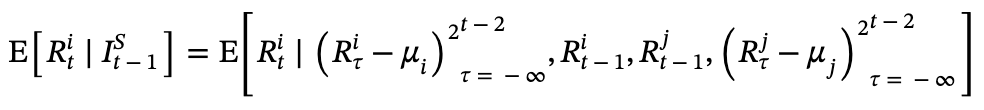
\includegraphics[scale=0.5]{granger_causality_1.png}
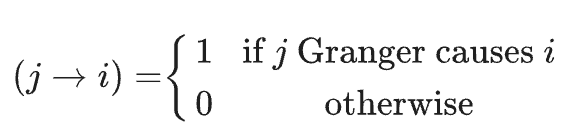
\includegraphics[scale=0.5]{granger_causality_2.png}

In general, if country \textit{j} causes volatility in country \textit{i}, then from \textit{j} to \textit{i} are connected in one direction. But, there is also a possibility in which country \textit{i} does not cause any volatility in country \textit{j}, indicating that the edge is only one direction. Lai \& Hu (2021) derived this formula to calculate the correlation of stock index volatility between two countries.

In another literature, Duan et al. (2020) were proposing to analyze covid recession systemic risk using both leverage and correlation factors. They were using $\Delta$CoVaR to calculate the leverage for each bank in pre-covid and post-covid eras based on evolution of their assets over time. $\Delta$CoVaR is a metric to calculate the growth rate of the market value of assets and firstly introduced in 2016 by Adrian and Brunnermeier. As the market value of banks’ assets change over time, so does their leverage level in the interbank networks thus affecting their activities and might expose them to looming systemic risk. The author derived the $\Delta$CoVaR equation based on the situation during covid outbreak and produce formula
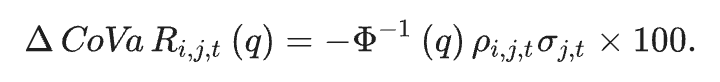
\includegraphics[scale=0.9]{covar.png}

This formula indicates that higher value of  $\Delta$CoVaR means higher systemic value for bank \textit{q}. The literature was using banks as the node and also using Granger-causality proposed by Billio et al. (2012) to determine connection between two banks.

\subsection{Centrality}
As previously indicated, there are at least four centrality approaches that are available in network science to do systemic risk analysis; degree, closeness, betweenness, and eigenvector. Each of these approaches has its own characteristics depending on the point of view that the network is representing.

For example, Lai \& Hu (2021) chose to use both degree and closeness centrality. As they build their network based on volatility correlation between countries, the higher the degree of a certain country means the higher the influence that particular country receives and emits. The authors also divided the degree into two categories that represent both the influence that countries take (in-degree) and also send out (out-degree), deepening the systemic risk analysis as it is not always reciprocal. What is interesting is that the authors’ reasoning on choosing the degree centrality as its first focus to do the analysis because it is the simplest centrality to be calculated yet brings sufficient preliminary information to the table. Due to the way authors constructed the network, the country with the highest in-degree held the most important information as they will be the country that is exposed the most by the systemic risk. On the other hand, the country with the highest out-degree can be seen as the largest domino piece that can potentially collapse the entire system if it falls. As further analysis, the authors also use closeness centrality to estimate the amount of time for systemic risk to propagate throughout the network. The country that has highest closeness centrality can reach out the furthest country in the network with only a few steps, meaning if this country collapses then the effect can be fastly transmitted. Although closeness centrality is prone to bias on loosely connected networks and generally more computational expensive compared to degree centrality, the authors argued that the network that they built was fully connected and small in terms of size (number of nodes). 

In contrast, Duan et al. (2020) and Markose et al. (2012) were using eigenvector centrality to analyze systemic risk in their bank network. The difference between these two literatures are Duan et al. (2020) were doing systemic risk analysis for covid recession scenario while Markose et al. (2012) were doing it for the 2007 great recession. In the authors’ network, the edges of the network have weights that represent the magnitude of the  $\Delta$CoVaR value. This is the main reason why the authors were using eigenvector centrality to measure systemic risk, as eigenvector is the only centrality measurement that takes strength of the weight into account. Unlike degree, closeness, and betweenness that focus on determining the centrality based on node’s attributes and locations, eigenvector centrality calculates the importance of the nodes based on the significance of all edges that connect to that particular node. By taking eigenvector values to determine the centrality, the authors successfully recreate the “too big to fail” doctrine in covid recession scenario, that was previously introduced by Adrian \& Brunnermeier (2016) in order to analyze the 2007 great recession. Nodes, in this case banks, that have high value of eigenvectors possess high systemic risk due to high leverage on their banking activities. In general, these nodes were big banks that had a lot of underlying assets providing them for bigger but high risk borrowed funds. Revealing these banks in the financial system will provide better understanding about potential cascading effects in case they are getting default. 

Additionally, another literature by Zhang et al. (2023) was also using  $\Delta$CoVaR value to build the network, but the authors were using global major indexes to create their network instead of global big banks. The authors were also using eigenvector centrality to measure systemic risk on their network, but they added closeness centrality as their preliminary information. The reasoning of the authors for this approach was the same as Lai \& Hu (2021). In fact, the authors were using that particular literature as their main reference when conducting the research.

Abuzayed et al. (2021) is also using  $\Delta$CoVaR to determine systemic risk in covid recession scenario, however they are not using any centrality approach to analyze the systemic risk. Therefore we will not discuss the author literature in this section.

\subsection{Clustering \& Modularity}

\section{Summary \& Conclusion}
This section will contain the summary from multiple approaches for systemic risk analysis in stock market

\section{Future Work}
This section will contain the potential future work for systemic risk analysis in stock market

%                Now build the reference list
\bibliographystyle{unsrt}   % The reference style
%                This is plain and unsorted, so in the order
%                they appear in the document.


\small
\bibliography{main}       % bib file(s).

\end{document}

